{\let\clearpage\relax\let\cleardoublepage\relax
\chapter{Modelli di formazione globali e semplificazioni introdotte}
}

\begin{workout}[Ref PPS]
Towarddeterminist model of planetary formation iV: effectsof type I migration
									: accumulation neare iceline
									: dynamical intaraction and coagulation of multiple rocky embrios (isolation mass, semi-analytic vs n-body)
									: eccentricity distribution of gas giant
Theoretical models of planetary system formation: mass vs. semi-major axis	(alibert carron 13)			Lecture 15 -planetary ...
Modelling planetary system formation with N-body simulation (11)
Global model of planet formation and evolution
Planetary population synthesis
planet population synthesis					
\end{workout}

\section{Modello disco di accrescimento e distribuzione condizioni iniziali}

Refs: Sec4 mordasini09

La popolazione planetaria \'e costruita risolvendo un modello di formazione planetaria pi\'u o meno realistico a partire da condizioni iniziali distribuite per rispecchiare le osservazioni e determinate da argomenti teorici.

\begin{workout}[modello globale: evoluzione dal semplice al complesso]
Global model of planets formation and evolution: more detailed submodels
\end{workout}

Il modello pi\'u semplice di disco di accrescimento usa distribuzione esponenziale per andamento densit\'a superficiale e temperature, assumendo disco otticamente sottile, e relazione $L_*\propto M_*^4$ di sequenza principale. Le lacune di questo modello sono che i dischi sono otticamente spessi con transizioni nell'opacit\'a, non \'e presente evoluzione temporale consistente.

Modelli pi\'u recenti  risolvono l'equazione per l'evoluzione viscosa:
\begin{align}
&\TDy{t}{\Sigma}=\frac{1}{r}\PDof{r}[3r\expy{1/2}\PDof{r}(\nu\Sigma r\expy{1/2})]+\dot{\Sigma}_w(r)+\dot{\Sigma}_p(r)\label{eq:diskaccrphev-m18}\\
&\dot{\Sigma}_w(a)=\left\{\begin{array}{c}0\\\frac{\dot{M}_w}{2\pi(a_{max}-R_g)a}\\\end{array}\right.
\end{align}
con $\dot{\Sigma}_w$ contributo della foto-evaporazione,  $\dot{\Sigma}_p$ contributo di accrescimento di gas dei pianeti e con densit\'a superficiale iniziale:
\begin{equation}
\Sigma(a,t=0)=\Sigma_0(\frac{r}{1AU})\expy{p_g}\Exp{[-(\frac{r}{R_o})\expy{2+p_g}]}(1-\sqrt{\frac{r}{R_i}})
\end{equation}
in i parametri possono essere scelti casualmente secondo una distribuzione di probabilit\'a ricavata dalle osservazioni.

La distribuzione di massa e la distribuzione della stima delle et\'a \'e mostrata in \ref{fig:initdistro}: la massa \'e determinata misurando flusso di emissione termica della polvera la distribuzione di $\log{M_{disk}}$  \'e gaussiana e per il cluster Ophiuchus la distribuzione \'e fittata da gaussiana con $\mu=-1.38$ ($M_{disk}=0.042\msun{}$) e $\sigma=0.49$.

Il tempo caratteristico del disco \'e determinato dalla viscosit\'a $\alpha$: fissata $\alpha$, e assumendo la distribuzione uniforme nel logaritmo di $\dot{M}_w$, e calcolando  $t_{disk}(\alpha,\Sigma_0,\dot{M}_w)$ si determinano gli estremi dello fotoevaporazione per riprodurre tempi di vita osservati.

 $t_{disk}(\alpha,\Sigma_0,\dot{M}_w)$ per $\dot{M}_w=\SIrange{5e-10}{3e-8}\msun{}/\si{\year}$ per $\alpha=\num{7e-3}$.



\begin{workout}[viscosit\'a disco]
Nella popolazione planetaria simulata $\alpha$ \'e fissato sulla base delle osservazioni  ed \'e omogeneo e costante.
\end{workout}

\begin{workout}[Modello di disco di accrescimento - (Mordasini18: 4) - Introduzione descrizione fenomeni grazie a PPS]
Refs: garaud lin 07, chiang goldreich 97
Un modello di disco  di accrescimento usato nelle simulazioni considera l'evoluzione della densit\'a superficiale tramite l'equazione \eqref{eq:diskaccrphev-m18}
\begin{align}
&\TDy{t}{\Sigma}=\frac{1}{r}\PDof{r}[3r\expy{1/2}\PDof{r}(\nu\Sigma r\expy{1/2})]+\dot{\Sigma}_w(r)+\dot{\Sigma}_p(r)\label{eq:diskaccrphev-m18}\\
&\dot{\Sigma}_w(a)=\left\{\begin{array}{c}0\\\frac{\dot{M}_w}{2\pi(a_{max}-R_g)a}\\\end{array}\right.
\end{align}
Densit\'a superficiale iniziale:
\begin{equation}
\Sigma(a,t=0)=\Sigma_0(\frac{r}{1AU})\expy{p_g}\Exp{[-(\frac{r}{R_o})\expy{2+p_g}]}(1-\sqrt{\frac{r}{R_i}})
\end{equation}
4-Mordasini18 (Hayashi81). $p_g\approx1$ (Andrews10).
\end{workout}

\section{Distribuzione iniziale planetesimi ed evoluzione}

Assumendo conversione completa di polvere in planetesimi, la densit\'a superficiale di planetesimi \'e
\begin{equation}
\Sigma_p(t=0,r)=f_{dg}\eta_{ice}\Sigma_g(t=0,r)
\end{equation}
con $f_{dg}$ rapporto gas/polvere (circa metallicit\'a) \'e una parametro casuale con distribuzione che riflette distribuzione di metallicit\'a stellari, $\eta_{ice}$ tiene conto della discontinuit\'a nella distribuzione superficiale di solidi all'iceline.

Sulla scorta della piccola differenza tra composizione solare e composizione meteoritica e assumendo inoltre che il ferro sia un buon indicatore della componente solida  si usa la formula
\begin{equation}
\frac{f_{D/G}}{f_{D/G\odot}}=10\expy{[\cel{Fe}{}{}{}/\cel{Fe}{}{}{}]}
\end{equation}

\begin{workout}[Planet host stars are enriched in nikel and silicon]
Robinson06
\end{workout}

Si introduce un fattore correttivo per il drift della polvere entro i \SI{20}{\astronomicalunit} compreso tra $2-4$ e infine si sfrutta la distribuzione della metallicit\'a per stelle di massa solare nelle vicinanze del Sole:
\begin{equation}
p([Fe/H])=\frac{1}{\sigma\sqrt{2\pi}}\exp{-\frac{([Fe/H]-\mu)^2}{2\sigma^2}}
\end{equation}
Per le stelle campionate da CORALIE si ha $\mu=-0.02$ e $\sigma=0.22$.

L'evoluzione della distribuzione dei planetesimi tiene conto dell'acrescimento sugli embrioni planetari:
\begin{equation}\dot{\Sigma}_p=-\frac{(3M_*)\expy{1/3}}{6\pi a_p^2B_LM_p\expy{1/3}}\dot{M}_c\end{equation}
e generalmente si assume che eccentricit\'a e inclinazione seguono distribuzione di Rayleigh.

Il drift dei planetesimi dovuto all'interazione col gas e la formaziane gap nella distribuzione dei planetesimi sono di solito trascurati.

\begin{workout}[Initial planetesimal distro]
Dust converted early everywhere fully-efficient (mordasini18: pg 12),Thommes pg8)
\begin{align*}
&\Sigma_p(t=0,r)=f_{dg}\eta_{ice}\Sigma_g(t=0,r)\\
&\dot{\Sigma}_p(r)=-\frac{1}{2\pi aB_LR_H}\dot{M}_c
\end{align*}
Icelines Mordasini 1141: inside where T exceeds sublimation
{Embryo starting position}
Usually a distro uniform in log(a): relative spacing of few Hill spheres (Kokubo Ida 10)
Ida, lin10: asymptotical isolation mass ''Toward a Deterministic Model of Planetary Formation VI'',
Trapped evolution model: Hasegawa pudritz 11, Cridland 16
\end{workout}

\section{Caratteristiche iniziali degli embioni planetarii e accrescimento}

La massa iniziale dei core deve essere molto minore della massa di isolamento: si usano core di frazioni di massa terrestre; la distanza dalla stella varia seguendo distribuzione di probabilit\'a $p(a)$ inversamente proporzionale alla distanza orbitale $p(a)\,da\propto\frac{da}{\Delta}\propto\,d\log{a}$. Il momento di comparsa \'e determinato dal rate di accrescimento dei planetesimi \eqref{eq:Gaccretionpl}.

La massa dei core varia per l'accrescimento dei planetesimi secondo
\begin{align}
&\dot{M}_c=\Omega\Sigma_pR^2_{capt}F_G
%&\dot{\Sigma}_p(r)=-\frac{1}{2\pi aB_LR_H}\dot{M}_c
\end{align}

Per determinare l'accrescimento di gas \'e necessario calcolare la struttura planetaria in alternativa si pu\'o averne una stima da
\begin{align}
&\dot{M}_{e,KH}=\frac{M_p}{\tau_{KH}}\\
&\tau_{KH}=10\expy{p}(\frac{M_p}{\mearth{}})^q(\frac{\kappa}{\si{\gram\per\square\cm}})\si{\year}
\end{align}
dove p,q sono ottenuti tramite modelli di struttura planetaria
\begin{workout}[Higher mass gap formation reduces accretion rate]
\begin{equation}
f_{va04}=1.668(\frac{M_p}{\mjupiter{}})\expy{1/3}\exp{-\frac{M_p}{1.5\mjupiter{}}}+0.04
\end{equation}
\end{workout}

\subsection{Parametrizzazioni della migrazione}

\begin{workout}[Migrazione mordasini 09]
La velocit\'a di migrazione calcolata per disco isotermo (\cite{tanaka2002}) \'e troppo rapida
\end{workout}


\begin{workout}[model migration-pps]
Tanaka02-m09
Paardekooper 11 - Dittkrist 14
\end{workout}

\begin{workout}[Lindblad torque: velocit\'a migrazione I]
masset casoli 10/paardekooper 10
\end{workout}

\begin{workout}[type I/type II transition]
m09: Hill radius larger than disk scale hight
\end{workout}

\begin{workout}[Saturation mass of horseshoe drag]
eq 2: theimportance of disk structure in stalling planet migration
\begin{equation}
\TDy{t}{r}=f(p,q,p_{\nu},p_{\xi})\frac{M_p}{M_*}\frac{\Sigma r^2}{M_*}(\frac{r\Omega}{c_s})^2r\Omega
\end{equation}
\end{workout}

\begin{workout}[Velocit\'a tipo II: viscosit\'a]
disk dominated
planet dominates: $\TDy{t}{a}=-\frac{3\nu}{a}\frac{\Sigma(a,t)a^2}{M_p}$
\end{workout}

\begin{workout}[Formation track and planet diversity]

\section{popolazioni sintetiche}
%Considero i risulati di alcuni modelli di formazione planetari (\cite{mordasini2018planetary}). 
La soluzione delle equazioni che descrivono l'accrescimento di massa dei protopianeti e la loro evoluzione orbitale interata su numerose combinazioni delle condizioni iniziali produce una popolazione di sistemi planetari appena formati dal disco-protoplanetario.

\begin{itemize}
\item Numerosi sistemi con piccola massa
\item Sistemi pianeti di piccola massa e giganti: sweet spot per pianeti giganti \'e all'esterno dell'ice-line.
\item Un pianeta gigante superstite di scattering trapianeti gignti vicini. Sistemi rari formati in dischi massicci con alta metallicit\'a
\end{itemize}•


\end{workout}

{\let\clearpage\relax\let\cleardoublepage\relax
\chapter{Confronto semi-quantitativo tra caratteristiche popolazioni sintetiche e osservate}
}

\section{Distribuzione popolazione sintetica diagramma $(a-M)$}

\begin{workout}[Diagramma $(a-M)$]

\begin{figure}[!ht]
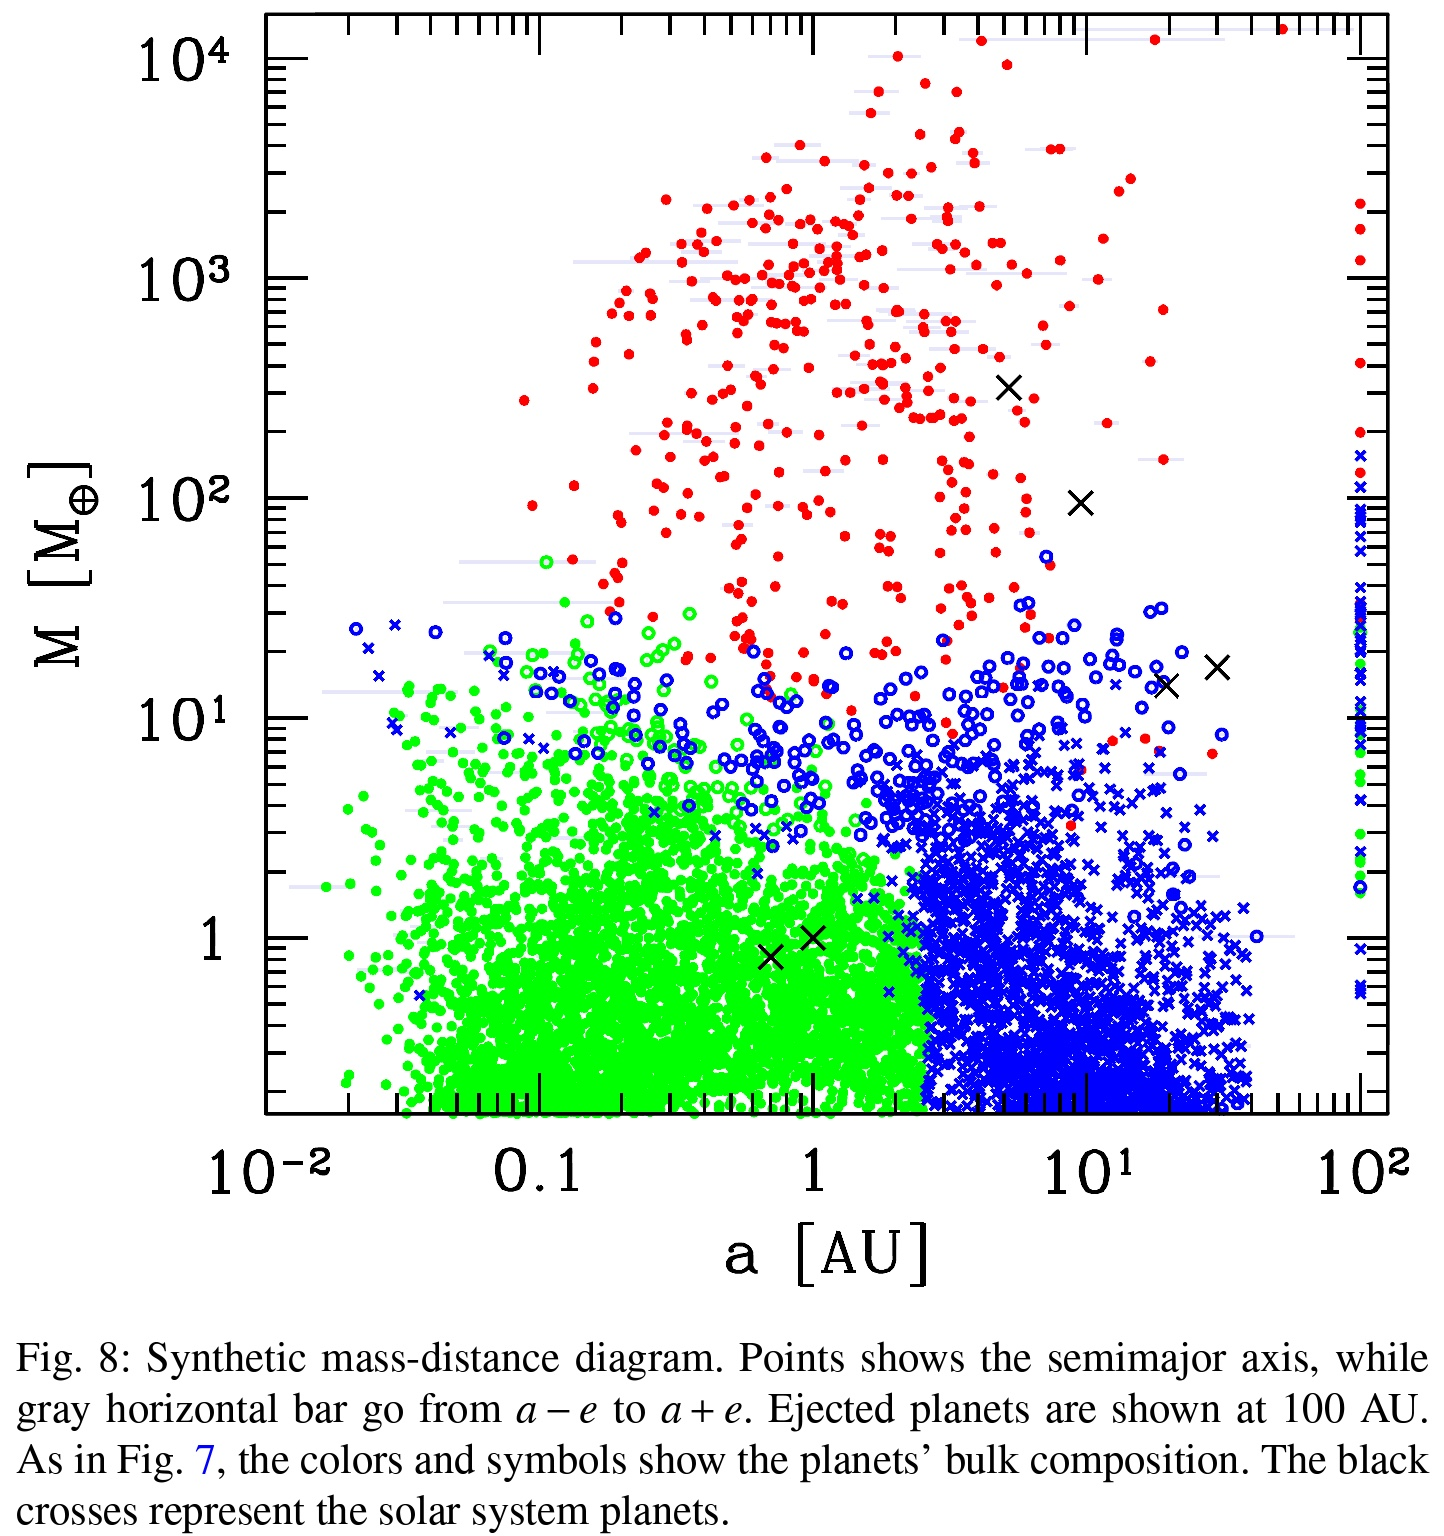
\includegraphics[width=0.9\textwidth,keepaspectratio]{ma-synth}
\caption{Da \cite{mordasini2018planetary}. Simulazione popolazione planetaria di 504 sistemi Punti rossi: pianeti giganti con $M_e/M_c>1$; blu hanno accresciuto core oltre la iceline, verdi all'interno dell'iceline .}
\end{figure}

La distribuzione della popolazione planetaria \'e mostrata in \ref{fig:MaLR-freq-synth}: la posizione finale di un pianeta \'e terminata principalmente dalla posizione iniziale e dai tempi caratteristici di accrescimento e migrazione; considerando inoltre l'interazione gravitazionale tra i pianeti si hanno effetti delle risonanze e eccitazione eccentricit\'a.

\begin{figure}[!ht]
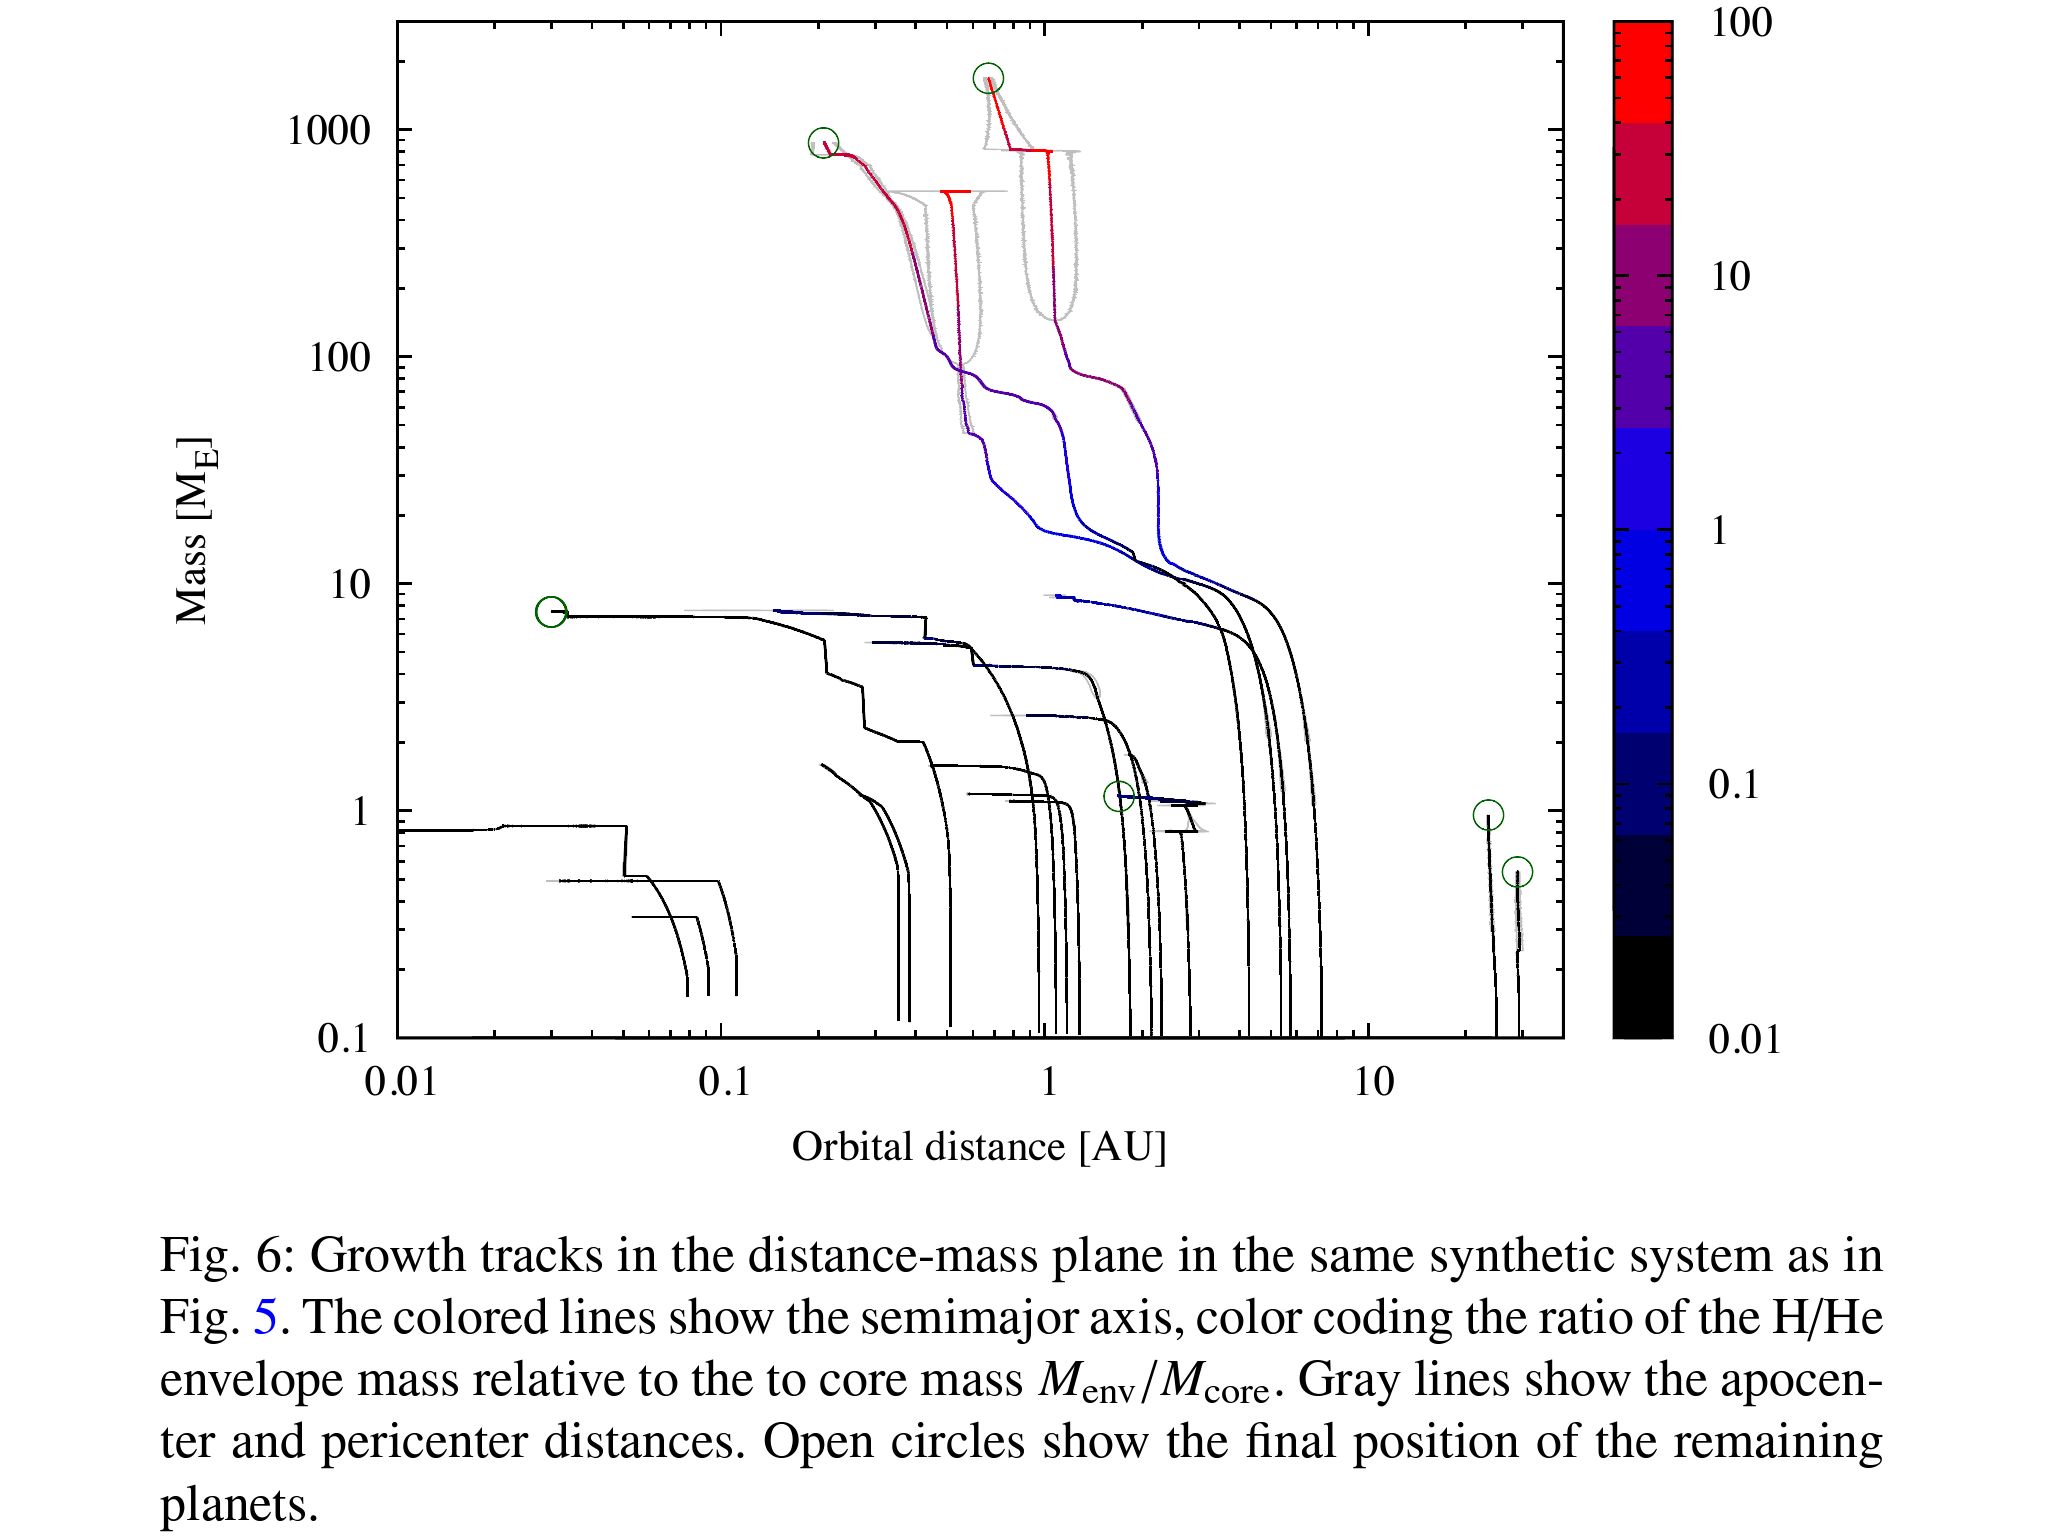
\includegraphics[width=0.9\textwidth,keepaspectratio]{track1}
\caption{Da \cite{mordasini2018planetary}. Formazione di un sistema planetario nel diagramma $a-M$: alla scomparsa del disco protoplanetario si hanno 2 pianeti giganti, un nettuniano caldo e 3 pianeti terrestri. La scala di colore indica la composizione $\frac{M_e}{M_c}$.}\label{fig:track1}
\end{figure}

Differenze con osservazioni

Nettuno/Saturno in posizioni poco affollate

Popolazione pianeti in origine nettuniani (frazione giaccio nel core $50\%$) che migrano all'interno accumulando materiale roccioso (frazione ghiaccio nel core $10-20\%$): saturazione momento di corotazione positivo.

\end{workout}

\begin{figure}[!ht]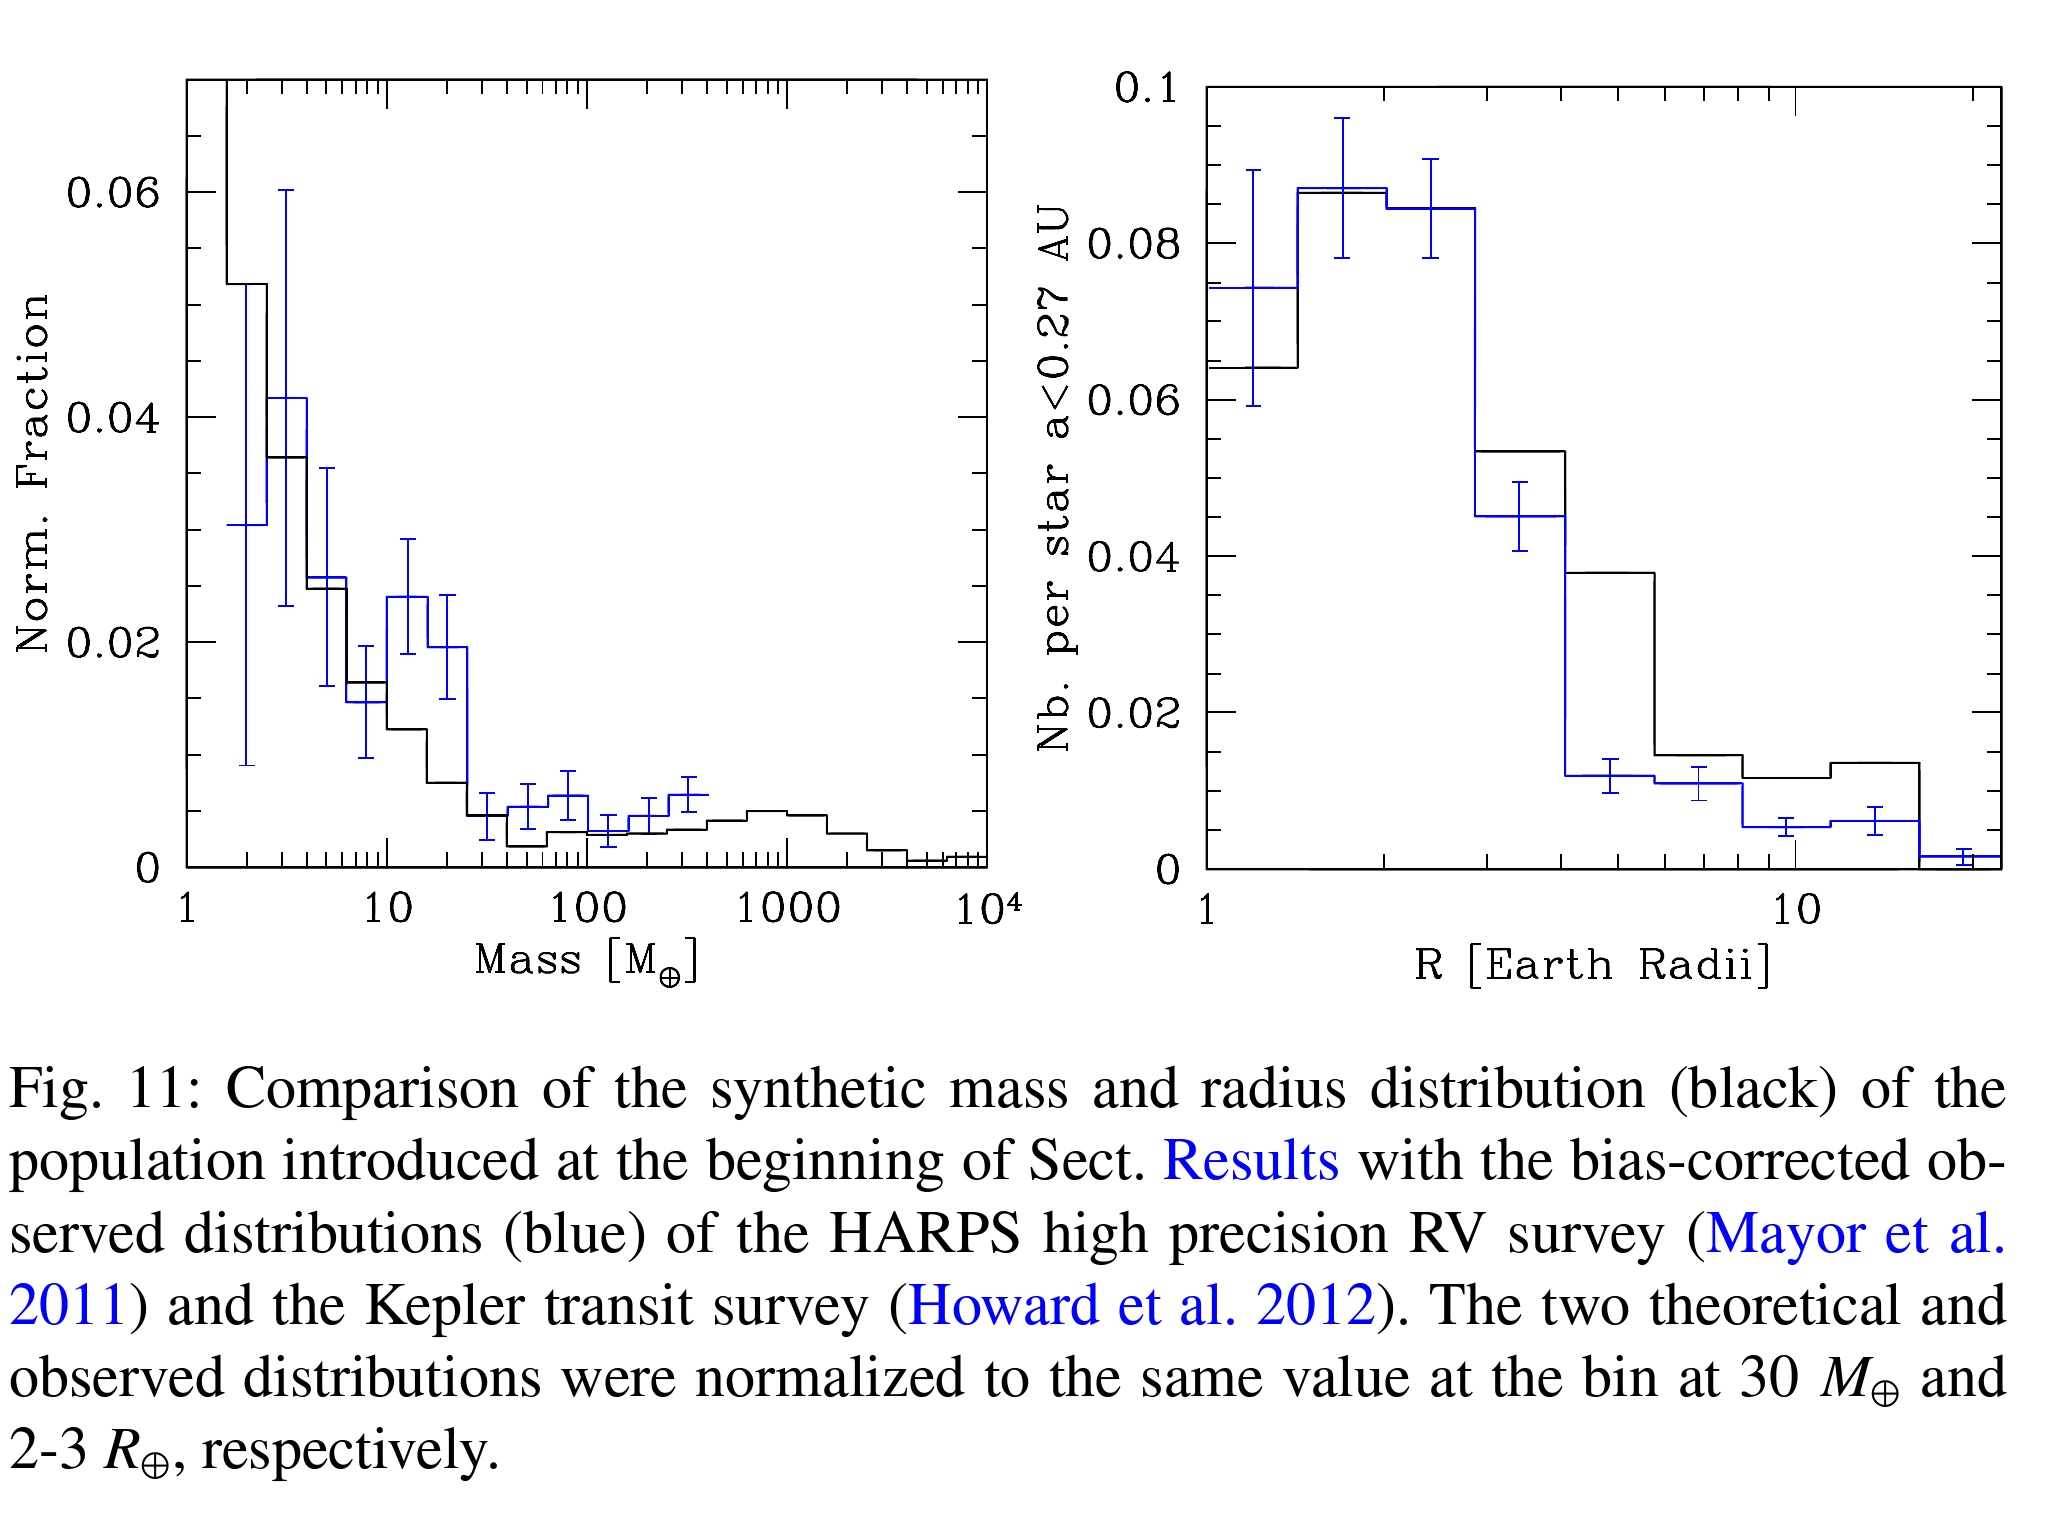
\includegraphics[keepaspectratio,width=0.9\textwidth]{MR-freq-obssynth}\label{}\caption{Da \cite{mordasini2018pèlanetary}.}\end{figure}

\begin{figure}[!ht]
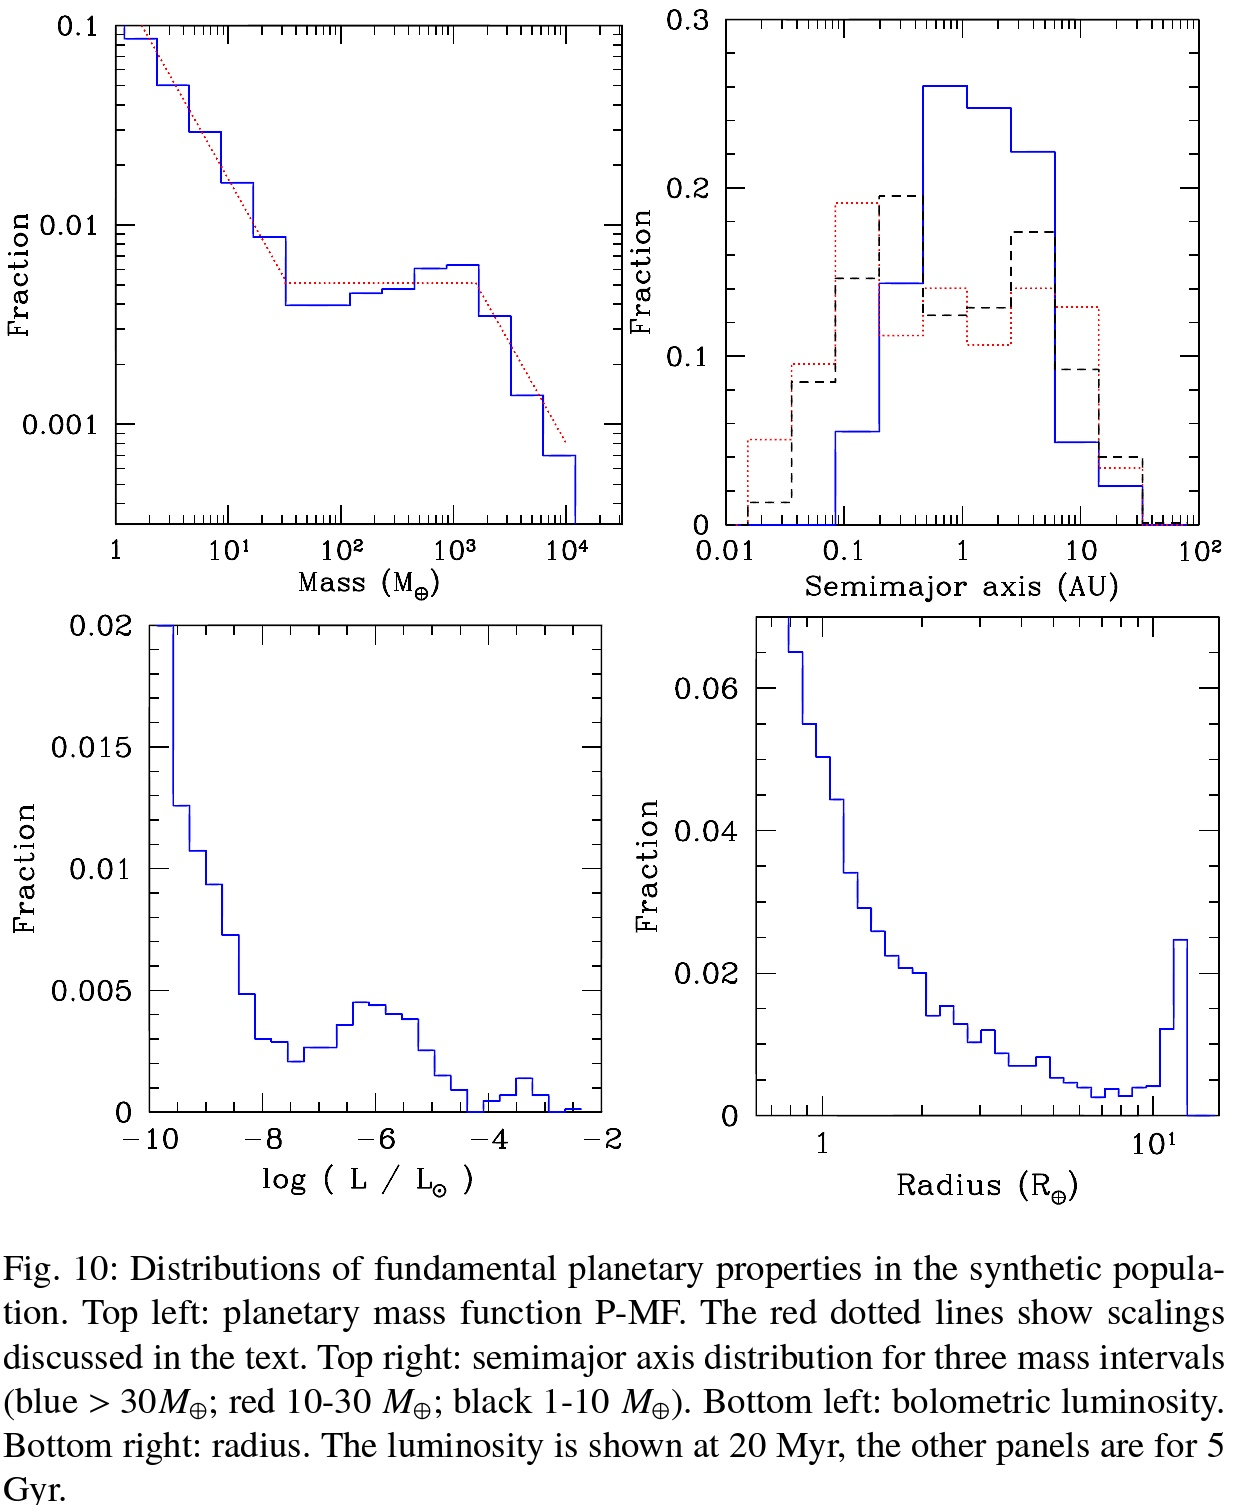
\includegraphics[width=0.9\textwidth,keepaspectratio]{MaLR-freq-synth}\label{fig:MaLR-freq-synth}
\caption{Da \cite{mordasini2018planetary}. }
\end{figure}

\begin{figure}[!ht]
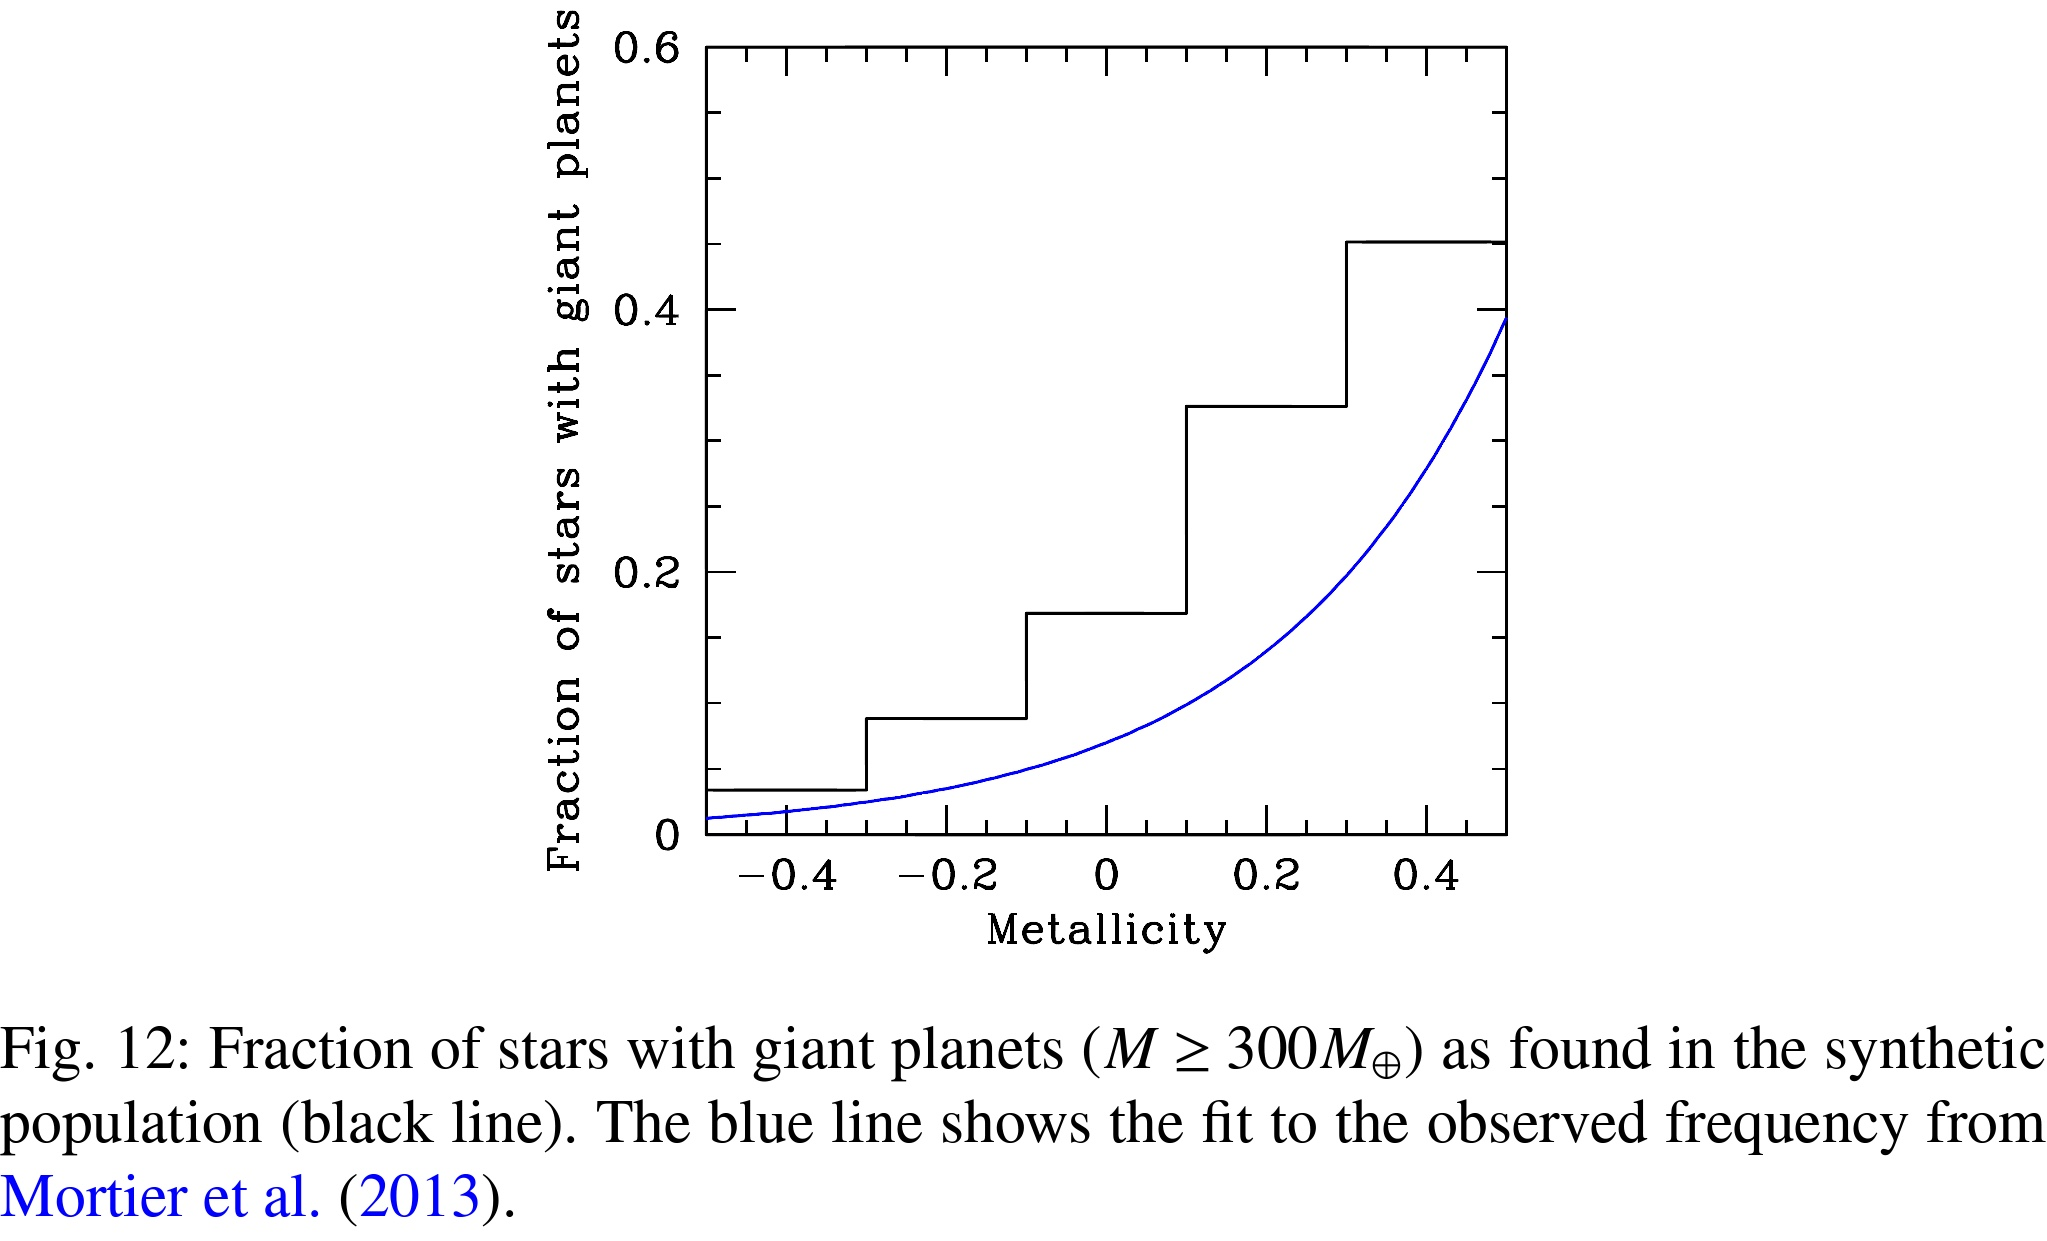
\includegraphics[width=0.9\textwidth,keepaspectratio]{giant-Zsynth}
\caption{Da \cite{mordasini2018planetary}. }
\end{figure}

\begin{figure}[!ht]
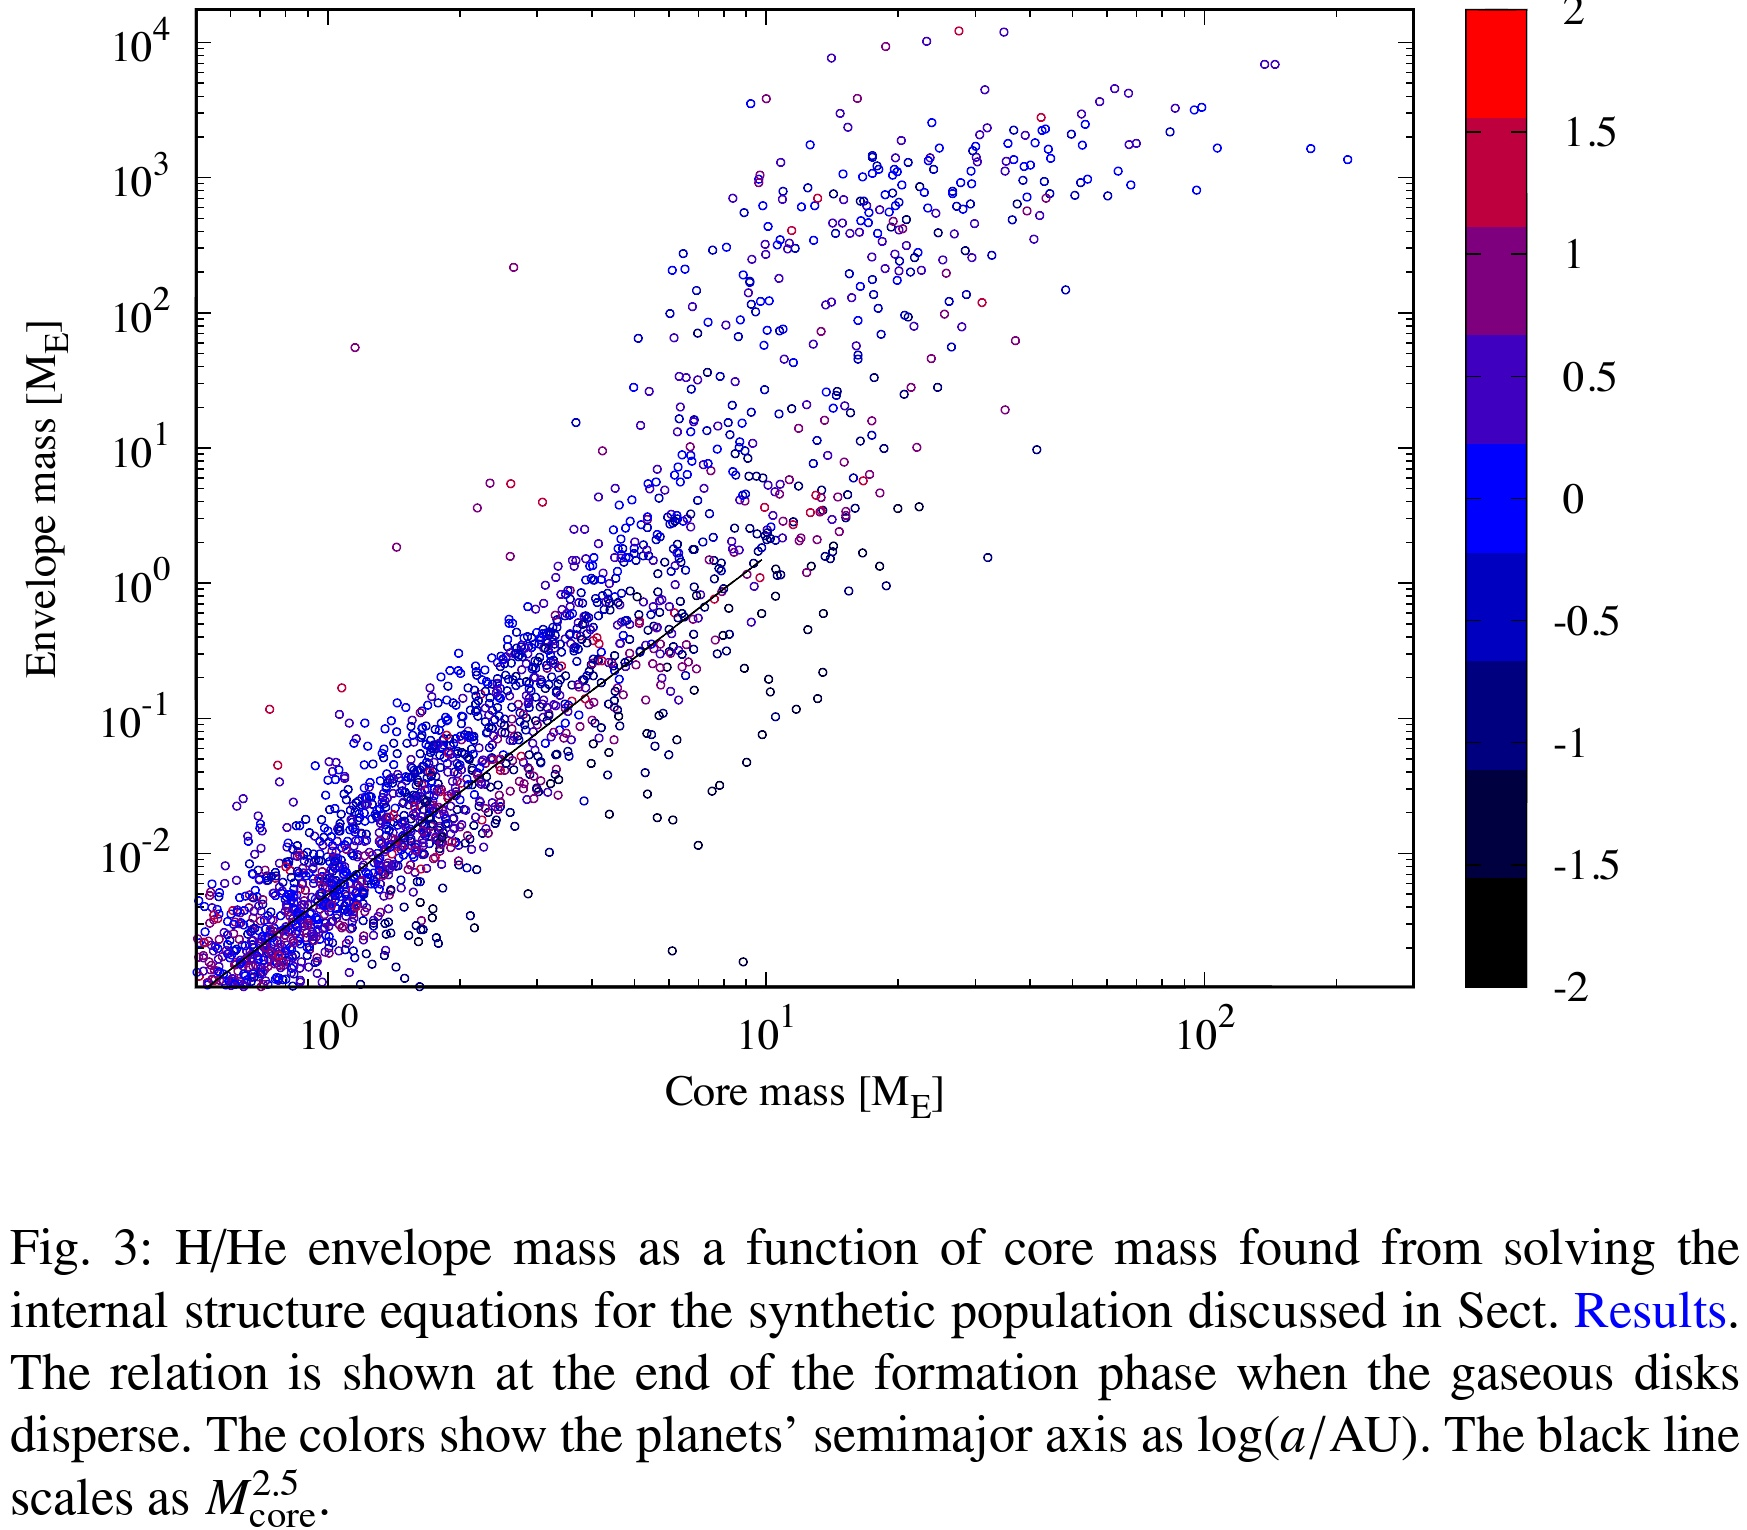
\includegraphics[width=0.9\textwidth,keepaspectratio]{envelopecoresynth}
\caption{Da \cite{mordasini2018planetary}. }
\end{figure}

{\let\clearpage\relax\let\cleardoublepage\relax
\chapter{Raffinamento dei modelli}
}


\begin{workout}[Effects of saturation, cooling and irradiation.]
Impact of planet migration model on planetary populations: effects of saturation, cooling and stellar irradiation (??)
Outward migration helps some planets to become massive, accumulation zone at certain semiaxis, at what mass corotation saturate?
Migration of protoplanets in radiative disks
\end{workout}
